\documentclass[8pt]{extarticle}
\title{}
\author{Avinash Iyer}
\date{}
\usepackage[shortlabels]{enumitem}

%font setup
%
\usepackage{newpxtext,eulerpx}

%paper setup
\usepackage{geometry}
\geometry{letterpaper, portrait, margin=1in}
\usepackage{fancyhdr}

%symbols
\usepackage{amsmath}
\usepackage{mathtools}
\usepackage{hyperref}
\usepackage{gensymb}

\usepackage[T1]{fontenc}
\usepackage[utf8]{inputenc}

%chemistry stuff
\usepackage[version=4]{mhchem}
\usepackage{chemfig}

%plotting
\usepackage{pgfplots}
\usepackage{tikz}
\tikzset{middleweight/.style={pos = 0.5, fill=white}}
\tikzset{weight/.style={pos = 0.5, fill = white}}
\tikzset{lateweight/.style={pos = 0.75, fill = white}}
\tikzset{earlyweight/.style={pos = 0.25, fill=white}}

%\usepackage{natbib}

%graphics stuff
\usepackage{graphicx}
\graphicspath{ {./images/} }

%code stuff
%when using minted, make sure to add the -shell-escape flag
%you can use lstlisting if you don't want to use minted
%\usepackage{minted}
%\usemintedstyle{pastie}
%\newminted[javacode]{java}{frame=lines,framesep=2mm,linenos=true,fontsize=\footnotesize,tabsize=3,autogobble,}
%\newminted[cppcode]{cpp}{frame=lines,framesep=2mm,linenos=true,fontsize=\footnotesize,tabsize=3,autogobble,}

\usepackage{listings}
\usepackage{color}
\definecolor{dkgreen}{rgb}{0,0.6,0}
\definecolor{gray}{rgb}{0.5,0.5,0.5}
\definecolor{mauve}{rgb}{0.58,0,0.82}

\lstset{frame=tb,
	language=Java,
	aboveskip=3mm,
	belowskip=3mm,
	showstringspaces=false,
	columns=flexible,
	basicstyle={\small\ttfamily},
	numbers=none,
	numberstyle=\tiny\color{gray},
	keywordstyle=\color{blue},
	commentstyle=\color{dkgreen},
	stringstyle=\color{mauve},
	breaklines=true,
	breakatwhitespace=true,
	tabsize=3
}
% text + color boxes
\usepackage{tcolorbox}
\tcbuselibrary{breakable}
\newtcolorbox{problem}[1]{colback = white, title = {#1}, breakable}
\newtcolorbox{solution}{colback = white, colframe = black!75!white, title = Solution, breakable}
%including PDFs
\usepackage{pdfpages}
\setlength{\parindent}{0pt}

\pagestyle{fancy}
\fancyhf{}
\rhead{Avinash Iyer}
\lhead{Applications of Graph Theory: Homework 1}
\begin{document}{
  \begin{problem}{Exercise 3}
    Suppose that four houses are under construction and each house must be provided with a connection of each of two utilities. Under the same conditions as the Three Houses and Three Utilities problem, can these conditions be satisfied for this Four Houses and Two Utilities Problem?
    \tcblower
    \begin{center}
      \begin{tikzpicture}
        \filldraw[blue] (-1,0) circle (2pt);
        \filldraw[red] (1,0) circle (2pt);
        \filldraw (0,1.5) circle (2pt)
        (0,0.5) circle (2pt)
        (0,-0.5) circle (2pt)
        (0,-1.5) circle (2pt);
        \draw (-1,0) -- (0,1.5);
        \draw (-1,0) -- (0,0.5);
        \draw (-1,0) -- (0,-1.5);
        \draw (-1,0) -- (0,-0.5);
        \draw (1,0) -- (0,1.5);
        \draw (1,0) -- (0,0.5);
        \draw (1,0) -- (0,-1.5);
        \draw (1,0) -- (0,-0.5);
      \end{tikzpicture}
    \end{center}
  \end{problem}
  \begin{problem}{Exercise 5}
    For the two polyhedra shown below, determine the number $V$ of vertices, the number $E$ of edges, and the number $F$ of faces. Show that the Euler Polyhedron Formula holds in each case.
    \begin{center}
      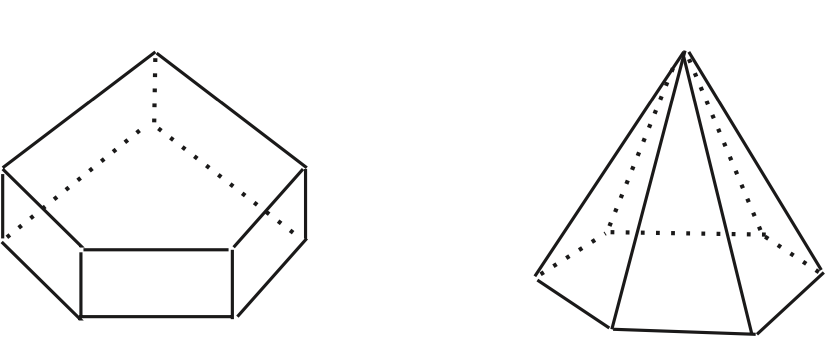
\includegraphics[width=5cm]{exercise_5}
    \end{center}
    \tcblower
    For the first polyhedron, we have $V = 10$, $E = 15$, $F = 7$, so $V-E+F = 2$.\\

    For the second polyhedron, we have $V = 7$, $E = 12$, and $F = 7$, so $V-E+F = 2$.
  \end{problem}
  \begin{problem}{Exercise 8a}
    Show that a knight's tour is not possible on a $4\times 4$ chessboard.
    \tcblower
    
  \end{problem}
}\end{document}
